
\documentclass[
    % -- opções da classe memoir --
    12pt,               % tamanho da fonte
    openright,          % capítulos começam em pág ímpar (insere página vazia caso preciso)
    twoside,            % para impressão em verso e anverso. Oposto a oneside
    a4paper,            % tamanho do papel. 
    % -- opções da classe abntex2 --
                   %chapter=TITLE,     % títulos de capítulos convertidos em letras maiúsculas
    %section=TITLE,     % títulos de seções convertidos em letras maiúsculas
    %subsection=TITLE,  % títulos de subseções convertidos em letras maiúsculas
    %subsubsection=TITLE,% títulos de subsubseções convertidos em letras maiúsculas
    % -- opções do pacote babel --
    english,            % idioma adicional para hifenização
    brazil              % o último idioma é o principal do documento
    ]{abntex2}

% ---
% Pacotes básicos 
% ---
\usepackage{lmodern}            % Usa a fonte Latin Modern          
\usepackage[T1]{fontenc}        % Selecao de codigos de fonte.
\usepackage[utf8]{inputenc}     % Codificacao do documento (conversão automática dos acentos)
\usepackage{lastpage}           % Usado pela Ficha catalográfica
\usepackage{indentfirst}        % Indenta o primeiro parágrafo de cada seção.
\usepackage{color}              % Controle das cores
\usepackage{graphicx}           % Inclusão de gráficos
\usepackage{microtype}          % para melhorias de justificação
\usepackage{pdflscape}
\usepackage{float}
\usepackage{tasks}
%\usepackage{subfigure}
% ---

\usepackage{xcolor}
\usepackage{listings}  

\lstset { %
	numbers=left,
    language=java,
    escapeinside={\%*}{*)},
    backgroundcolor=\color{black!5},
	basicstyle=\ttfamily\scriptsize,
    keywordstyle=\color{blue}\ttfamily,
    stringstyle=\color{red}\ttfamily,
    commentstyle=\color{red}\ttfamily,
    breaklines=true,
    morecomment=[l][\color{magenta}]{\#}
}
\lstdefinelanguage{XML}
{
  %morestring=[b]",
  morestring=[s]{>}{<},
  morecomment=[s]{<?}{?>},
  stringstyle=\color{black},
  identifierstyle=\color{blue},
  keywordstyle=\color{cyan},
	showstringspaces=false,
  morekeywords={xmlns,version,type}% list your attributes here
}


\renewcommand{\lstlistingname}{Listagem}
    
% ---
% Pacotes adicionais, usados apenas no âmbito do Modelo Canônico do abnteX2
% ---
\usepackage{lipsum}             % para geração de dummy text
% ---

% ---
% Pacotes de citações
% ---
\usepackage[brazilian,hyperpageref]{backref}     % Paginas com as citações na bibl
\usepackage[alf]{abntex2cite}   % Citações padrão ABNT


% alterando o aspecto da cor azul
\definecolor{blue}{RGB}{41,5,195}

% informações do PDF
\makeatletter
\hypersetup{
        %pagebackref=true,
        pdftitle={\@title}, 
        pdfauthor={\@author},
        pdfsubject={\imprimirpreambulo},
        pdfcreator={LaTeX with abnTeX2},
        pdfkeywords={abnt}{latex}{abntex}{abntex2}{trabalho acadêmico}, 
        colorlinks=true,            % false: boxed links; true: colored links
        linkcolor=blue,             % color of internal links
        citecolor=blue,             % color of links to bibliography
        filecolor=magenta,              % color of file links
        urlcolor=blue,
        bookmarksdepth=4
}
\makeatother

% --- 
% Espaçamentos entre linhas e parágrafos 
% --- 

% O tamanho do parágrafo é dado por:
\setlength{\parindent}{1.3cm}

% Controle do espaçamento entre um parágrafo e outro:
\setlength{\parskip}{0.2cm}  % tente também \onelineskip

% ---
% compila o indice
% ---
\makeindex
% ---
\graphicspath{{images/}} %Pasta padrão das imagens
% ----
% Início do documento
% ----
\begin{document}

	%Arquivo de Capa
\newpage
\begin{figure}[!htp]
  \includegraphics[scale = 0.4]{unesp-logo.png}  %logo da UNESP
\end{figure}

\hspace*{73mm}
\begin{minipage}{79mm}
	\vskip-35mm
	\begin{center}
		UNIVERSIDADE ESTADUAL PAULISTA \\[-2mm] "JÚLIO DE MESQUITA FILHO" \\[-2mm] Campus de Presidente Prudente
	\end{center}
\end{minipage}
\begin{center}
	{\large Fundação de Amparo à Pesquisa do Estado de São Paulo (FAPESP)  }
\end{center} 
%nome do autor
\vspace*{30mm}
\begin{center}
	{\large Uso de \textit{Business Process Model} como apoio à condução e à replicação de experimentos controlados em Engenharia de Software 
  }
\end{center}

\vspace*{15mm}

\begin{center}
	{\large RELATÓRIO CIENTÍFICO PARCIAL  }\\
\end{center}



{\flushleft
	{\normalsize
		\vspace{30mm}
		\hrulefill\\
		%\hspace{10mm} \textbf{Título: }Uso de \textit{Business Process Model} como apoio à condução e à replicação de experimentos controlados em Engenharia de Software \\
		\hspace{10mm} \textbf{Bolsista: }Leandro Ungari Cayres\\
		\hspace{10mm} \textbf{Orientador: }Prof. Dr. Rogério Eduardo Garcia\\
		%\hspace{10mm} \textbf{Orgão Financiador: }Fundação de Amparo à Pesquisa do Estado de São Paulo (FAPESP)\\
		\hspace{10mm} \textbf{Processo: }2015/18238-9\\
		\hspace{10mm} \textbf{Período do relatório: }01/12/2016 a 31/05/2017\\
		\hspace{10mm} \textbf{Vigência: }01/12/2016 a 30/11/2017 \\
		\hrulefill\\
	}
}

\vspace*{\fill}

\begin{center}
	Presidente Prudente \\Maio de 2017  %local da tortura e data da entrega do plágio
\end{center}

  \pagenumbering{roman}
	
	\newpage	
	\tableofcontents 
	\newpage
	\listoffigures 
	\newpage
	\listoftables 
	\newpage
		

	\chapter*{Resumo}

\addcontentsline{toc}{section}{Resumo}

O conjunto de dados  relativos aos procedimentos, artefatos, resultados e conclusões de um experimento controlado deve ser mantido em Pacotes de Laboratório. Contudo, há relatos na literatura de dificuldades de compreensão em relação ao plano de execução do experimento, devido à ausência de informações explícitas de sua estrutura, mesmo quando baseada na ontologia \textit{ExperOntology}. Tal fato impacta negativamente a replicação ou mesmo a condução de um experimento, não permitindo uma visão geral sobre o estudo. Nesse contexto, o presente estudo propõe a utilização de modelos de processo de negócio para a modelagem de protocolos de experimentação, utilizando a notação gráfica BPMN, e sua incorporação ao Pacote de Laboratório. Assim, neste relatório são apresentadas as atividades para adequar  uma ferramenta de modo a permitir a construção de modelos de processo de negócio para a representação do protocolo do experimento em um Pacote de Laboratório. Adicionalmente, a ferramenta contribui para a portabilidade e transferência de instâncias de Pacotes de Laboratório, facilitando a legibilidade e integração por  utilizar de um modelo não-relacional orientado a documentos (XML). Neste texto também é apresentada a proposta para renovação da bolsa de iniciação científica.
	\clearpage
	
  \textual
	\pagenumbering{arabic}
	\chapter{Introdução}

Este relatório tem como objetivo apresentar as atividades desenvolvidas pelo bolsista Leandro Ungari Cayres referente ao projeto  registrado junto à FAPESP com número 2016/17477-2, sob orientação do Prof. Dr. Rogério E. Garcia, período compreendido entre dezembro de 2016 a maio de 2017.

O objetivo geral deste projeto consiste em prover uma interface capaz de apresentar visualmente o protocolo de um experimento, utilizando a notação BPM (\textit{Business Process Modeling}). Ou seja, deve-se: (1) prover ao experimentador a possibilidade de planejar seu experimento utilizando a notação BPM e; (2) prover ao replicador a possibilidade de visualizar o protocolo contido no PL, também utilizando a notação BPM.

Como objetivo específico, considera-se a modificação da camada de apresentação (interface) da ferramenta \textit{OntoExpTool}, incorporando o modelo gráfico BPM à ferramenta, assim como as adequações necessárias na camada de controle. É importante ressaltar que objetiva-se constituir um sistema de software que permita a concepção e a troca de pacotes de laboratórios, para apoiar a condução de experimentos controlados.

Como questões de investigação (em nível de Iniciação Científica), tem-se: o uso de BPM contribui para a definição do protocolo de experimentos? Quais recursos devem ser utilizados para o uso da tecnologia? Como suplantar limitações para a tecnologia a ser utilizada?

Para apresentar as atividades desenvolvidas até o momento, este relatório encontra-se dividido em $5$ capítulos, além desta introdução:

\begin{itemize}

\item No capítulo \ref{cp:engenharia} é apresentada uma breve revisão sobre Engenharia de Software Experimental, com foco em experimentos controlados, para contextualização do projeto de pesquisa.

\item No capítulo \ref{cp:bpmn} é descrito um breve histórico da notação BPM, assim como, apresentando os elementos que compõem este notação.

\item No capítulo \ref{cp:prototipo} é apresentado o andamento das atividades de implementação da interface de modelagem.

\item No capítulo \ref{ch:plano_atividades} é apresentado o plano de atividades inicial para o projeto. É, também, apresentado o que fora cumprido até o presente momento, bem como as atividades que serão efetuadas a partir desta etapa.

\item Por fim, no Capítulo \ref{cp:conclusoes} são apresentadas as considerações finais do presente relatório.
\end{itemize}
     


	
	\chapter{Processo Experimental: seus dados e metadados}
\label{cp:engenharia}

A Engenharia de Software Experimental busca medir e avaliar modelos e tecnologias em contextos práticos, objetivando a obtenção de um corpo de conhecimento. Porém, resultados oriundos de um único experimento não podem estabelecer tal corpo de conhecimento, de modo a determinar fatos sobre um dado fenômeno devido às mais diversas variações que podem ser introduzidas no processo experimental, tais como influências culturais~\cite{Basili99, Miller:2005, Shull03}. Perante a isto, se faz necessário que dados sobre estudos independentes sejam armazenados e compartilhados.

O ato de experimentação consiste no centro do processo científico, a qual representa uma atividade na área de pesquisa científica e se utiliza de métodos de investigação experimental para a condução de experimentos~\cite{Travassos02}. 

Segundo \citeauthoronline{Basili99}~(\citeyear{Basili99}), a experimentação ajuda a determinar a eficácia de métodos e de teorias propostas. Somente experimentos verificam as teorias, podem explorar os fatores críticos, e dar luz ao fenômeno novo para que as teorias possam ser formuladas e corrigidas.

A execução de um experimento requer uma sequência de atividades estabelecidas previamente, que por meio das quais seja possível conduzir um processo experimental de forma precisa e sistemática. Desse modo, \citeauthoronline{Wohlin2012}~(\citeyear{Wohlin2012}) propõem as seguinte organização em fases: 
\begin{itemize}
\item \textbf{Definição} –- estabelece quais são os problemas tratados;
\item \textbf{Planejamento} -– determina-se o projeto, instrumentação e os possíveis riscos para validação dos resultados;
\item \textbf{Operação} –- coleta-se os dados do experimento;
\item \textbf{Análise e Interpretação} –- os dados são analisados e avaliados;
\item \textbf{Apresentação e Empacotamento} -– os resultados são apresentados e suas informações são armazenadas para uso futuro.
\end{itemize}

%\textbf{Definição} -- estabelece quais são os problemas tratados; \textbf{Planejamento} -- determina-se o projeto, instrumentação e os possíveis riscos para validação dos resultados; \textbf{Operação} -- coleta-se os dados do experimento; \textbf{Análise e Interpretação} -- os dados são analisados e avaliados; \textbf{Apresentação e Empacotamento} -- os resultados são apresentados e suas informações são armazenadas para uso futuro. 

Na Figura~\ref{ideia} é apresentado um gráfico com o processo de experimentação adaptado de~\citeauthoronline{Wohlin2012}~(\citeyear{Wohlin2012}): nela é possível observar as fazes, assim como tarefas inerentes a cada uma. 

\begin{figure}[!ht]
\centering
\includegraphics[width=0.98\textwidth]{images/Experimentacao.pdf}
\caption{Processo de Experimentação -- adaptado de~\cite{Wohlin2012}.}
\label{ideia}
\end{figure}

Como apoio, os estudos experimentais atuam como ferramentas para obtenção dos dados necessários através de todo o processo de desenvolvimento de software, almejando resultados objetivos e significativos de forma a alcançar melhorias no processo. Também segundo~\citeauthoronline{Wohlin2012}~(\citeyear{Wohlin2012}), tais estudos podem ser divididos nas seguintes categorias:

\begin{itemize}

\item Pesquisa de opinião: neste primeiro tipo de estudo experimental, busca-se obter dados a respeito de uma técnica ou ferramenta específica, seja uma análise qualitativa ou quantitativa, por meio de entrevistas ou questionários aplicados a uma amostra capaz de representar uma determinada população. Nesta categoria, não controle de execução ou medidas.

\item Estudos de caso: esta categoria é voltada ao monitoramento de atividades, projetos ou tarefas visando observar um atributo específico, ou estabelecer relações entre alguns destes, a qual se prolonga por um determinado período de tempo. Por se tratar uma atividade observacional, o nível de controle é mais elevado do que o anterior.

\item Experimentos controlados: por fim, nesta categoria, o estudo experimental tem sua execução manipulada de forma direta e sistemática, a fim de se ter controle sob todos os elementos que o compõem. Podem ser efetuados experimentos controlados em ambiente universitário, de forma a reduzir custos e riscos do que aplicá-los diretamente à indústria.

\end{itemize}

Somente experimentos verificam as teorias, podem explorar os fatores críticos, e dar luz ao fenômeno novo para que as teorias possam ser formuladas e corrigidas. O processo experimental proporciona de modo sistemático, disciplinado, e controlada a avaliação de processos e de atividades humanas~\cite{Travassos02}.

Através da replicação de experimentos, pesquisadores adquirem conhecimento adicional a respeito dos conceitos estudados. Para que se possa replicar experimentos, é necessário que seu empacotamento seja realizado apropriadamente. Uma replicação em contextos diferentes sujeita o experimento a variações, dentre os quais fatores humanos, socioeconômicos e ambientais do âmbito que o experimento é realizado, possibilitando maior precisão na verificação da validade de hipóteses~\cite{Shull03}. E para a replicação de um experimento, tanto intra quanto extra-grupo~\cite{Mendonca08}, é de suma importância a organização do registro das atividades de um experimento controlado, que são mantidas no chamado \textit{Pacote de Laboratório}.

%%%%%%%%%%%%%%%%%%%%%%%%%%%%%%%%%%%%%%%%
%%%%%%%%%%%%%%%%%%%%%%%%%%%%%%%%%%%%%%%%

\section{Pacotes de Laboratório}
\label{sec:Pacote}
Dentro do âmbito da Engenharia de Software Experimental, a todo momento diversas pesquisas, técnicas e ferramentas são desenvolvidos para validar teses ou otimizar soluções, porém tais recursos ou informações isoladas não formam um corpo de
conhecimento consistente, faz-se necessário compartilhá-los entre os grupos de pesquisa por meio do uso de pacotes de laboratório.

A condução de experimentos controlados ou de suas respectivas replicações, ambas necessitam de validação. A execução destes experimentos, tanto no papel de experimentador quanto de replicador, podem influenciar de forma positiva ou negativa sob muitos aspectos, principalmente em relação ao nível de experiência do condutor do experimento. Por fim, o conjunto de informações obtidos através da execução do processo experimental compõem uma nova instância de pacote de laboratório~\cite{Garcia08}.

Diversos pesquisadores relatam dificuldades na revisão de pacotes de laboratório, como problemas no compartilhamento de conhecimento entre grupos de pesquisa devido uma falta de padronização para a integração de um conhecimento novo e/ou isolado ao conhecimento comum~\cite{Scatalon11}. Desta forma, é imprescindível uma boa definição e construção
de um pacote de laboratório com o uso de uma estrutura específica de simples compreensão, possibilitando inclusive o uso de ontologias para seu desenvolvimento.


%Garcia et al. 
\citeauthoronline{Garcia08} (\citeyear{Garcia08}) propõem o uso de uma ontologia para apoiar a atividade de \textit{Empacotamento} processo de Experimentação no contexto de Engenharia de Software, que descreve os conceitos que compõem um pacote de laboratório para experimentos controlados, chamada \textit{ExperOntology}, apresentada na Figura~\ref{fig:onto01}.
Uma ontologia é uma especificação formal explícita de uma conceitualização compartilhada, definindo parte de um domínio por meio de termos relevantes e seus respectivos relacionamentos, cuja estruturação é baseada por determinadas regras. As regras (axiomas) da \textit{ExperOntology} não são apresentados aqui, mas podem ser observados em~\cite{Garcia08}.
\begin{figure}[!ht]
\centering
\includegraphics[width=0.8\textwidth]{images/controlados.png}
\caption{Ontologia para Experimentos Controlados~\cite{Garcia08}.}\label{fig:onto01}
\end{figure}

\begin{figure}[!htb]
\centering
\includegraphics[width=\textwidth]{images/onto.png}
\caption{Ontologia para Pacotes de Laboratório~\cite{Garcia08}.}\label{fig:onto02}
\end{figure}

A \textit{ExperOntology} visa a definir o principais conceitos de experimentos controlados desde a fase de definição até a análise de resultados, sendo importante ressaltar a evolução do experimento e o uso de pacotes de laboratório para armazenamento~\cite{Garcia08}. 

Na Figura \ref{fig:onto02} estão descritos os conceitos que devem fazer parte de um pacote de laboratório, segundo a \textit{ExperOntology}. Inicialmente, é definido um propósito, um contexto, um objeto de estudo e o foco a serem considerados no estudo controlado; en seguida, é elaborada de uma hipótese inicial, a qual juntamente com uma objeto de estudo e um contexto formam a formalização da hipótese. A partir deste ponto, são definidas as hipóteses nulas e alternativas, assim como as variáveis dependentes e independentes. Durante a fase de planejamento, são determinados os objetos de experimentação como as tecnologias e artefatos sob investigação.

O principal objetivo das fases de definição e planejamento é estabelecer um modelo experimental que satisfaça todos os requisitos para a fase de análise. O resultado destas fases culmina em um modelo experimental e no plano de execução, o qual permite a definição de um ambiente controlado, realização de testes das hipóteses e minimização de ameaças para a validação do experimento.

Todos os conceitos apresentados devem ser mantidos no Pacote de Laboratório e, portanto, devem ser instanciados em uma base de dados ou outro meio equivalente para persistir os dados.

\section{Bancos de Dados Não-Relacionais}

Diversas tecnologias para armazenamento de dados têm sido propostas para a persistência de dados, como os Sistemas Gerenciadores de Banco de Dados (\textit{SGBDs}).

O modelo relacional de dados tem sido utilizado em larga escala desde a sua criação. Este modelo tem como característica a utilização de tabelas e tuplas para o armazenamento de dados, assim como o uso de chaves primárias para garantia de unicidade (identificação única de elementos de dados)~\cite{brito2010bancos}.

Mediante ao crescente número de aplicações, o volume de dados tem aumentado exponencialmente nos últimos anos, e com tal crescimento limitações do modelo relacional tem ficado evidente, principalmente quanto à eficiência na recuperação de dados e escalabilidade~\cite{toth2011abordagem}. Para este projeto, a principal limitação é a necessidade de se ter uma estrutura de tabelas pré-definidas, com seus respectivos atributos, o que pode ser uma restrição, pois experimentos controlados podem ter variações nos dados tratados, difícil de ser acomodados em uma estrutura relacional.

Como alternativa, há soluções tecnológicas alternativas que priorizam flexibilidade quanto ao armazenamento, desse modo, não empregam regras presentes no modelo relacional tradicional. Um dessas alternativas é o Modelo Não-Relacional (NoRel), o qual não tem como objetivo substituir o modelo relacional por completo, mas somente em casos em que seja mais vantajoso utilizá-lo, como em ambientes de Big Data. Alguns representantes de base não-relacionais são: Cassandra~\cite{cassandra2014apache}, Dynamo~\cite{sivasubramanian2012amazon}, MongoDB~\cite{banker2011mongodb} e BigTable~\cite{chang2008bigtable}.

Devido à inexistência de regras para a organização dos seus dados, diversas categorias de sistemas de banco de dados não-relacionais tem sido desenvolvidas, os principais são detalhados a seguir.


\begin{itemize}
\item Orientados a Colunas (\textit{Column}): é a categoria que mais se aproxima do modelo relacional, porém todas as suas operações são voltadas para as colunas, ao invés das tuplas como no modelo relacional. O seu grande diferencial está na facilidade de inserção de novas colunas, ou seja, atributos com o sistema já em operação, conforme se tornarem necessários, sem apresentar problemas de esquema ou redundância de dados~\cite{vaish2013getting}.

\item Armazenamento em Documentos (\textit{Document}): nesta categoria cada item é armazenado em um novo arquivo, em geral sua organização é feita através de estruturas chamadas coleções as quais são equivalentes as tabelas no modelo relacional, não possuem qualquer esquema, dois objetos de uma mesma coleção podem ter atributos diferentes, o que permite grande flexibilidade, sendo que cada registro é um arquivo. Os principais formatos de arquivos são JSON, XML, BSON e YAML~\cite{vaish2013getting}.

\item Armazenamento Chave/Valor (\textit{Key/Value}): também muito semelhante à categoria anterior (\textit{Document}), porém seu armazenamento é feito com uso de uma chave, assemelhando-se a uma tabela \textit{Hash}, ou um \textit{array} associativo. Sua grande vantagem é busca por chaves~\cite{vaish2013getting}.

\item Armazenamento em Grafos (\textit{Graph}): esta categoria tem foco nos relacionamentos entre as entidades, que no caso são os nós do grafo, permitindo o uso de múltiplas ligações entre os nós para demonstrar características em comum. Este modelo pode ser ideal para redes sociais. Uma prática usual é a mescla entre o banco de dados orientado a documentos e o orientado a grafos, tornando não obrigatória a presença de relacionamentos~\cite{vaish2013getting}.

\end{itemize}

\begin{table}[!htb]
\centering
\caption{Banco de Dados Não-Relacional e sua tecnologia de armazenamento.}\label{tab:01}
\begin{tabular}{c|c|c|c|c}
\hline
\textbf{Document} & \textbf{Key-Value} & \textbf{XML} & \textbf{Column} & \textbf{Graph}\\ 
\hline                               
MongoDB & Redis & BaseX & BigTable & Neo4J \\
\hline
CouchDB & Membase & eXist & Haddop/HBase & FlockDB \\
\hline
RavenDB & Voldemort & - & Cassandra & InfiniteGraph \\
\hline
\end{tabular}
\end{table}
\normalsize

Na Tebela~\ref{tab:01} há uma breve lista de tecnologias de banco de dados não-relacionais e a respectiva classificação, segundo as classes de armazenamento apresentadas.
Antes de se estabelecer uma comparação entre os modelos, é importante definir conceitos como que deem compor essa comparação, são eles:



\begin{itemize}
\item Escalonamento: este conceito, no contexto de banco de dados, consiste na capacidade em que uma base de dados tem de destruição tanto horizontal (\textit{scale out}), neste caso a estruturação do sistema é dividida em várias máquinas tanto por parte do banco de dados; quanto vertical (\textit{scale up}), no qual são realizadas melhorias de hardware em relação à processamento e armazenamento~\cite{toth2011abordagem}.

\item Consistência: refere-se à capacidade de manter os dados de forma íntegra, de modo que evite quaisquer problemas no banco de dados possam modificar ou corromper os dados armazenados~\cite{brito2010bancos}.

\item Disponibilidade: este quesito se refere a capacidade de acesso do usuário a referida informação, tanto em quesito de velocidade quanto de solicitação~\cite{brito2010bancos}.
\end{itemize}

\begin{table}[!bth]
\label{comparativo}
\centering
\caption{Análise Comparativa do Modelo Relacional e Não-Relacional~\cite{brito2010bancos}.}
\begin{tabular}{l|p{5.7cm}|p{5.7cm}}
\hline
 & \textbf{Relacional} & \textbf{Não-Relacional} \\ 
\hline                               
\textbf{Escalonamento} & Possível, porém complexo devido à natureza estruturada do modelo, a adição de forma dinâmica e transparente de novos nós no modelo não é realizada de modo natural. & Uma das principais vantagens desse modelo, por não possuir nenhum tipo de esquema predefinido, o modelo possui maior flexibilidade o que favorece a inclusão transparente de outros elementos.\\
\hline
\textbf{Consistência} & Ponto mais forte do modelo relacional. As regras de consistência presentes propiciam uma maior grau de rigor quanto à consistência das informações. & Realizada de modo eventual no modelo: só garante que, se nenhuma atualização for realizada sobre o item de dados, todos os acessos a esse item devolvem o último valor atualizado. \\
\hline
\textbf{Disponibilidade} & Dada a dificuldade de se conseguir trabalhar de forma eficiente com a distribuição dos dados, esse modelo pode não suportar a demanda muito grande de informações do banco. & Outro fator fundamental do sucesso desse modelo. O alto grau de distribuição dos dados propicia que um maior número de solicitações aos dados seja atendida por parte do sistema e que o sistema fique menos tempo não-disponível. \\
\hline
\end{tabular}
\normalsize
\end{table}

Por fim, de modo a esclarecer as reais vantagens e desvantagens do uso de uma base de dados não-relacional, na Tabela~\ref{comparativo} é apresentado um comparativo com o tradicional modelo relacional analisando os quesitos de consistência, escalonamento e disponibilidade~\cite{brito2010bancos}.

Perante esta conceituação, a camada de persistência será elaborada utilizando o banco de dados \textit{MySQL}~\cite{mysql2001mysql} devido à utilização da ferramenta \textit{OntoExpTool}~\cite{Pucci2014}, mantendo assim a compatibilidade para os modelos já criados. Para a persistência da camada de interface será utilizada uma estrutura orientada a documentos, utilizando \textit{eXtensible Markup Language} (XML). Tal decisão foi tomada pois a estrutura orientada a documentos  se mostrou adequada tanto para o armazenamento, quanto para a transferência de protocolos experimentais entre exterimentador e replicador. Adicionalmente, essa organização estrutural permite que os dados de um experimentos sejam mantidos em uma base de dados. e seu protocolo, expresso em BPMN (armazenado em XML) possa ser compartilhado, sem expor os dados. O compartilhamento do protocolo juntamente com os dados do experimento (dados coletados) podem ser compartilhados, desde que desejado pelo experimentador (resposável pela criação do experimento e, consequentemente, do seu Pacote de Laboratório).

	
	\chapter{Pacotes de Laboratório}
\label{cp:pacotes}
No âmbito da Engenharia de Software Experimental, diversas pesquisas, técnicas e ferramentas têm sido  desenvolvidos para avaliar modelos ou otimizar soluções. Porém, tais recursos ou informações isoladas não formam um corpo de conhecimento consistente, então tornando necessário compartilhá-los entre os grupos de pesquisa por meio do uso de pacotes de laboratório.

A condução de experimentos controlados e suas respectivas replicações são organizadas em um \textit{framework} proposto por~\citeauthoronline{mendoncca2008framework}~(\citeyear{mendoncca2008framework}). O nível de experiência do condutor do experimento, tanto no papel de experimentador quanto de replicador, influencia a qualidade do estudo experimental e deve ser considerada na análise do experimento (talvez como uma ameaça). O conjunto de informações obtido a partir da execução do processo experimental compõe uma nova instância de pacote de laboratório~\cite{Garcia08}.

Diversos pesquisadores relatam dificuldades na revisão de pacotes de laboratório, como problemas no compartilhamento de conhecimento entre grupos de pesquisa devido à falta de padronização para a integração de um conhecimento novo e/ou isolado ao conhecimento comum~\cite{Scatalon11}. Desse modo, é imprescindível a definição e a construção de um pacote de laboratório com o uso de uma estrutura de simples compreensão. O uso de ontologias para sua estruturação é uma alternativa para facilitar a transferência de conhecimento inter e intra-grupos. A \textit{ExperOntology} foi proposta para a organização de Pacotes de Laboratório e é descrita na Seção~\ref{exper}.

\section{Modelo para Melhoria da Experimentação}
\label{fire}

\citeauthoronline{mendoncca2008framework}~(\citeyear{mendoncca2008framework}) apresentaram um modelo para o processo de experimentação (FIRE – \textit{Framework for Improving the Replication of Experiments}), apresentado na Figura~\ref{image:fire}, que objetiva o gerenciamento do conhecimento e a melhoria de replicações de experimentos controlados em Engenharia de Software.

\begin{figure}[!htb]
\centering
\includegraphics[width=\textwidth]{images/fire.png}
\caption{Ciclos do processo \textit{FIRE}~\cite{mendoncca2008framework}.}\label{image:fire}
\end{figure}

Inicialmente, o ciclo de \textit{Execução do Experimento} corresponde à execução do experimento em estudo. O ciclo de \textit{Aprendizado Intra-Grupo} representa o aprendizado, empacotamento e planejamento de novos experimentos por um mesmo grupo de pesquisadores, visando a construir um corpo de conhecimento local. As atividades desse ciclo consistem em:

\begin{itemize}
\item Definição das metas do experimento.
\item Planejar o experimento, identificar participantes e obter artefatos para a preparação do experimento.
\item Execução do experimento.
\item Instanciação e evolução de Pacotes de Laboratório, armazenando a experiência adquirida.
\end{itemize}

O ciclo de \textit{Aprendizado Inter-Grupo} objetiva a padronização do Pacote de Laboratório, a evolução do pacote de experimentação e o compartilhamento de conhecimento entre os grupos de pesquisa, visa a construir um amplo corpo de conhecimento sobre um tema baseado em replicações executadas por diferentes grupos de pesquisa. As atividades chave
são:

\begin{itemize}
\item Planejamento e coordenação das atividades experimentais entre grupos.
\item Compreensão dos pacotes de laboratório e dos resultados experimentais inter-grupo.
\item Compartilhamento e consolidação do aprendizado com outros grupos.
\item Padronização do conhecimento adquirido pelos grupos de pesquisa.
\item Criação e aprimoramento do corpo de conhecimento.

\end{itemize}

A externalização e internalização do conhecimento na forma de pacotes de laboratório e a concretização do conhecimento externo aos pacotes de laboratório são os pontos críticos do processo \textit{FIRE}. A ausência de diretrizes que apoiem o registro e manutenção de informações explícitas, e a referencia de pacotes de laboratório como corpo de informação explícita sobre um experimento para alcançar uniformidade necessária entre replicações são mencionados na literatura. Entretanto, o \textit{FIRE} não aborda como solucionar tais problemas, assim como não indica outros mecanismos que possam apoiar de modo adequado a evolução do conhecimento~\cite{Garcia06}.


%%%%%%%%%%%%
\section{\textit{ExperOntology}}
\label{exper}
Na Ciência da Computação, o termo ontologia foi introduzido inicialmente por~\citeauthoronline{gruber1995toward}~(\citeyear{gruber1995toward}), que a definiu como ``uma especificação explícita de uma conceitualização''. Posteriormente, uma reformulação foi proposta por~\citeauthoronline{borst1997construction}~(\citeyear{borst1997construction}) acrescentando a perspectiva colaborativa: ``Uma ontologia é uma especificação formal e explícita de uma conceitualização compartilhada''. Quando representado de maneira formal, o corpo do conhecimento se baseia em uma conceitualização explícita ou implícita, sendo composto por objetos, conceitos, outras entidades e as suas relações existentes na área de interesse. Tal conceitualização é considerada uma visão simplificada e abstrata do mundo representado para atingir algum dado objetivo~\cite{rautenberg2016processo}. 
Adicionalmente, uma ontologia é uma especificação formal explícita de uma conceitualização compartilhada, definindo parte de um domínio por meio de termos relevantes e seus respectivos relacionamentos, cuja estruturação é baseada por determinadas regras. 


\citeauthoronline{Garcia08}~(\citeyear{Garcia08}) propõem o uso de uma ontologia para apoiar a atividade de \textit{Empacotamento} no contexto de Engenharia de Software, a qual descreve os conceitos que compõem um pacote de laboratório para experimentos controlados, chamada \textit{ExperOntology}, apresentada em seu nível de abstração mais alto na Figura~\ref{fig:onto01}.


A \textit{ExperOntology} baseia-se no conhecimento de pesquisadores e na experiência em condução de experimentos controlados, principalmente na avaliação das técnicas V\&V (Validação e Verificação). É composta por dois níveis de refinamento, sendo que o primeiro se refere aos principais conceitos de experimento controlado, enquanto o segundo trata do refinamento dos conceitos e do pacote de laboratório. Na condução de um experimento original, é gerado um pacote de laboratório, assim como no processo de replicação.

\begin{figure}[!ht]
\centering
\includegraphics[width=0.9\textwidth]{images/controlados.png}
\caption{Ontologia para Experimentos Controlados~\cite{Garcia08}.}\label{fig:onto01}
\end{figure}

A ontologia proposta por~\citeauthoronline{Garcia08}~(\citeyear{Garcia08}) visa a definir o principais conceitos de experimentos controlados desde a fase de definição até a análise de resultados, sendo importante ressaltar a evolução do experimento e o uso de pacotes de laboratório para armazenamento. 

\begin{figure}[!htb]
\centering
\includegraphics[width=\textwidth]{images/onto.png}
\caption{Ontologia para Pacotes de Laboratório~\cite{Garcia08}.}\label{fig:onto02}
\end{figure}

Na Figura~\ref{fig:onto02} são definidos os conceitos para um pacote de laboratório. Inicialmente, a hipótese inicial de um experimento controlado é definida, sendo constituída pelo objeto de estudo, de acordo com o propósito, sob o foco da qualidade e um contexto específico. Um exemplo de utilização de como um conceito instanciado é utilizado em múltiplas  fases do processo de um experimento, é o conceito \textit{Hipótese Formalizada}:

\begin{itemize}
\item Na atividade \textit{Definição}, a medida que o objetivo do experimento é definido, a base para formulação das hipóteses também é estabelecida, incluindo a \textit{Hipótese Inicial}.
\item Durante a atividade Planejamento, servirá de base para a criação das \textit{Hipóteses Formalizadas} (Hipótese Nula e Hipótese Alternativa). Após a criação das \textit{Hipóteses Formalizadas}, o experimentador estabelece a \textit{Variável Independente} e \textit{Variável Dependente}.
\item Durante a atividade \textit{Operação}, os tratamentos são aplicados aos sujeitos, ou seja, o experimento tem sua execução iniciada.
\item Após o término da execução, ainda na atividade \textit{Operação}, é conveniente que o experimentador aplique uma validação dos dados. Isso ocorre por meio da verificação e validação dos dados informados pelos participantes, para que os resultados do experimento sejam válidos, e para tanto, as \textit{Hipóteses Formalizadas} são ser consultadas.
\end{itemize}


Em seguida, na atividade \textit{Análise e Interpretação}, durante os \textit{Testes de Hipóteses}, as \textit{Hipóteses Formalizadas} passam por avaliação para que seja verificado qualquer possibilidade de rejeição de uma hipótese nula. Hipóteses e conclusões são armazenadas no pacote de laboratório~\cite{Pucci2014}. 

Todos os conceitos apresentados devem ser mantidos no Pacote de Laboratório. Quando se uma ferramenta computacional como apoio ao \textit{Empacotamento}, os conceitos podem ser persistidos em uma base de dados ou outro meio equivalente.


\section{Bancos de Dados Não-Relacionais}

Diversas tecnologias para armazenamento de dados têm sido propostas para a persistência de dados, como os Sistemas Gerenciadores de Banco de Dados (\textit{SGBDs}).

O modelo relacional de dados tem sido utilizado em larga escala desde a sua criação. Esse modelo tem como característica a utilização de tabelas e tuplas para o armazenamento de dados, assim como o uso de chaves primárias para garantia a unicidade (identificação única de elementos de dados)~\cite{brito2010bancos}.

Mediante o crescente número de aplicações, o volume de dados tem aumentado exponencialmente nos últimos anos, e com tal crescimento limitações do modelo relacional têm ficado evidente, principalmente quanto à eficiência na recuperação de dados e escalabilidade~\cite{toth2011abordagem}. Para este projeto, a principal limitação é a restrição de estruturas de tabelas pré-definidas, com seus respectivos atributos, trata-se de um fator limitante, pois experimentos controlados podem ter variações nos dados tratados, difícil de ser acomodados em uma estrutura relacional.

Como alternativa, há soluções tecnológicas que priorizam flexibilidade quanto ao armazenamento, desse modo, não empregam regras presentes no modelo relacional tradicional. Um dessas alternativas é o Modelo Não-Relacional (NoRel), cujo objetivo não é substituir o modelo relacional, mas utilizá-lo em casos em que seja mais vantajoso admitindo a falta de rigidez nas estruturas de dados, como em ambientes de Big Data. Alguns representantes de base não-relacionais são: Cassandra~\cite{cassandra2014apache}, Dynamo~\cite{sivasubramanian2012amazon}, MongoDB~\cite{banker2011mongodb} e BigTable~\cite{chang2008bigtable}.

Devido à inexistência de regras para a organização dos seus dados, diversas categorias de sistemas de banco de dados não-relacionais tem sido desenvolvidas, os principais são detalhados a seguir.

\begin{itemize}
\item Orientados a Colunas (\textit{Column}): é a categoria que mais se aproxima do modelo relacional, porém todas as suas operações são voltadas para as colunas, ao invés das tuplas, como no modelo relacional. O seu grande diferencial está na facilidade de inserção de novas colunas, ou seja, novos atributos com o sistema já em operação, conforme se tornarem necessários, sem apresentar problemas de esquema ou redundância de dados~\cite{vaish2013getting}.

\item Armazenamento em Documentos (\textit{Document}): nessa categoria cada item é armazenado em um novo arquivo, em geral sua organização é feita por meio de estruturas chamadas \textit{Coleções} as quais são equivalentes as tabelas no modelo relacional, não possuem qualquer esquema, dois objetos de uma mesma coleção podem ter atributos diferentes, o que permite grande flexibilidade, sendo que cada registro é um arquivo. Os principais formatos de arquivos são JSON, XML, BSON e YAML~\cite{vaish2013getting}.

\item Armazenamento Chave/Valor (\textit{Key/Value}): também muito semelhante à categoria anterior (\textit{Document}), porém seu armazenamento é feito com uso de uma chave, assemelhando-se a uma tabela \textit{Hash}, ou um \textit{array} associativo. Sua grande vantagem é busca por chaves~\cite{vaish2013getting}.

\item Armazenamento em Grafos (\textit{Graph}): esta categoria tem foco nos relacionamentos entre as entidades, que no caso são os nós do grafo, permitindo o uso de múltiplas ligações entre os nós para demonstrar características em comum. Esse modelo pode ser ideal para redes sociais. Uma prática usual é a mescla entre o banco de dados orientado a documentos e o orientado a grafos, tornando não obrigatória a presença de relacionamentos~\cite{vaish2013getting}.

\end{itemize}

\begin{table}[!htb]
\centering
\caption{Banco de Dados Não-Relacional e sua tecnologia de armazenamento.}\label{tab:01}
\begin{tabular}{c|c|c|c|c}
\hline
\textbf{Document} & \textbf{Key-Value} & \textbf{XML} & \textbf{Column} & \textbf{Graph}\\ 
\hline                               
MongoDB & Redis & BaseX & BigTable & Neo4J \\
\hline
CouchDB & Membase & eXist & Haddop/HBase & FlockDB \\
\hline
RavenDB & Voldemort & - & Cassandra & InfiniteGraph \\
\hline
\end{tabular}
\end{table}
\normalsize

Na Tabela~\ref{tab:01} há uma lista sucinta de tecnologias de banco de dados não-relacionais e a respectiva classificação, segundo as classes de armazenamento apresentadas.
Antes de se estabelecer uma comparação entre os modelos, é importante definir conceitos como que deem compor essa comparação, são eles~\cite{toth2011abordagem,brito2010bancos}:

\begin{itemize}
\item Escalonamento: este conceito, no contexto de banco de dados, consiste na capacidade de distribuição tanto horizontal (\textit{scale out}), neste caso a estruturação do sistema é dividida em várias máquinas tanto por parte do banco de dados; quanto vertical (\textit{scale up}), no qual são realizadas melhorias de hardware em relação ao processamento e ao armazenamento.

\item Consistência: refere-se à capacidade de manter os dados de forma íntegra, de modo que evite inconsistências no banco de dados que corrompam os dados armazenados.

\item Disponibilidade: esse quesito se refere à capacidade de acesso do usuário à referida informação, tanto em quesito de velocidade, quanto de solicitação.
\end{itemize}

\begin{table}[!bth]

\centering
\caption{Análise Comparativa do Modelo Relacional e Não-Relacional~\cite{brito2010bancos}.}
\label{tabela:comparativo}
\begin{tabular}{l|p{5.7cm}|p{5.7cm}}
\hline
 & \textbf{Relacional} & \textbf{Não-Relacional} \\ 
\hline                               
\textbf{Escalonamento} & Possível, porém complexo devido à natureza estruturada do modelo, a adição de forma dinâmica e transparente de novos nós no modelo; não é realizada de modo natural. & Uma das principais vantagens desse modelo, por não possuir nenhum tipo de esquema predefinido, o modelo possui maior flexibilidade; o que favorece a inclusão transparente de outros elementos.\\
\hline
\textbf{Consistência} & Ponto mais forte do modelo relacional. As regras de consistência presentes propiciam uma maior grau de rigor quanto à consistência dos dados. & Realizada de modo eventual no modelo: só garante que, se nenhuma atualização for realizada sobre o item de dados, todos os acessos a esse item devolvem o último valor atualizado. \\
\hline
\textbf{Disponibilidade} & Dada a dificuldade de se conseguir trabalhar de forma eficiente com a distribuição dos dados, esse modelo pode não suportar a demanda muito grande de informações do banco. & Outro fator fundamental do sucesso desse modelo. O alto grau de distribuição dos dados propicia que um maior número de solicitações aos dados seja atendida por parte do sistema e que o sistema fique menos tempo não-disponível. \\
\hline
\end{tabular}
\normalsize
\end{table}

Por fim, de modo a esclarecer as reais vantagens e desvantagens do uso de uma base de dados não-relacional, na Tabela~\ref{tabela:comparativo} é apresentado um comparativo com o tradicional modelo relacional analisando os quesitos de consistência, escalonamento e disponibilidade~\cite{brito2010bancos}. 

\section{Considerações Finais}
Como apresentado neste capítulo, a condução de processos experimentais de modo isolado não é capaz de solidificar um corpo de conhecimento, faz-se necessário a avaliação de modelos, técnicas e ferramentas sob diferentes perspectivas e níveis de experiência. Desse modo, foi apresentado o arcabouço de atividades denominado \textit{FIRE}~\cite{mendoncca2008framework}, que visa ao aprimoramento do conhecimento oriundo de experimentos. Adicionalmente, foi apresenta uma ontologia denominada \textit{ExperOntology}, a qual descreve o conjunto de conceitos para a formalização de um pacote de laboratório em experimentos controlados. Porém a qualidade do pacote instanciado está atrelado diretamente à tecnologia utilizada em sua concepção. Desse modo, apresentam-se com grande viabilidade base de dados não-relacionais orientadas a documentos, devido a eliminação de diversos regras de integridade, além de prover maior flexibilidade de dados, em detrimento às bases de dados relacionais.
	
	\chapter{Modelagem de Processo de Negócio}
\label{cp:bpmn}

Para a elaboração dos modelos de processos de negócio, é relevante o conhecimento de todos os elementos envolvidos na execução de processos, tais como atores, clientes internos e externos, recursos e limitações; por meio dos quais é estabelecido um modelo que propicia um melhor entendimento, organização e representação, seja esta uma visão contextual abstrata ou com alto nível de detalhamento, conforme necessário. 

Tipicamente, a representação de um modelo de processos inclui ícones, que representam atividades, eventos, decisões, condições e outros elementos do processo \cite{brazil2011bpm}. Esses elementos podem conter informações sobre os relacionamentos entre eles e com o ambiente, bem como sobre o comportamento de cada elemento na cadeia de processos.

\section{\textit{Business Process Modeling and Notation}}

A especificação da notação BPMN foi elaborada e lançada em 2004 pelo Instituto de Gerenciamento de Processos de Negócio ou BPMI (\textit{Business Process Management Institute}), que realizou fusão ao Consórcio OMG. Posteriormente, a notação BPMN foi adotada pelo Consórcio OMG como o padrão para modelagem de processos. Após a padronização, foram lançadas algumas versões subsequentes, atualmente encontrando-se na versão 2.0 \cite{object2016business}.

Segundo \citeauthoronline{correia2015enhancing}~(\citeyear{correia2015enhancing}), \textit{Business Process Modeling and Notation} (BPMN) é atualmente a notação de modelagem de processos de negócio mais usada entre profissionais da área, devido a sua flexibilidade e abrangência. Consiste em uma tecnologia recente e pode ser utilizada por profissionais com diferentes níveis de conhecimento técnico. A formalização dos conceitos de modelagem de processos de negócio é baseada em um metamodelo construído a partir da linguagem \textit{Unified Modeling Language} (UML). 

A construção de processos de negócio através desta notação, utiliza um conjunto de padrões denominado ``metamodelo para definição de processos de negócio'' \cite{object2016business}. Nesse sentido, a especificação BPMN provê uma notação gráfica para representar processos de negócio por meio de um diagrama chamado ``diagrama de processo de negócio''. Esse diagrama é elaborado a partir de um conjunto de elementos gráficos que compõem diagramas simples de serem desenvolvidos e
compreendidos. 

\begin{figure}[!ht]
\centering
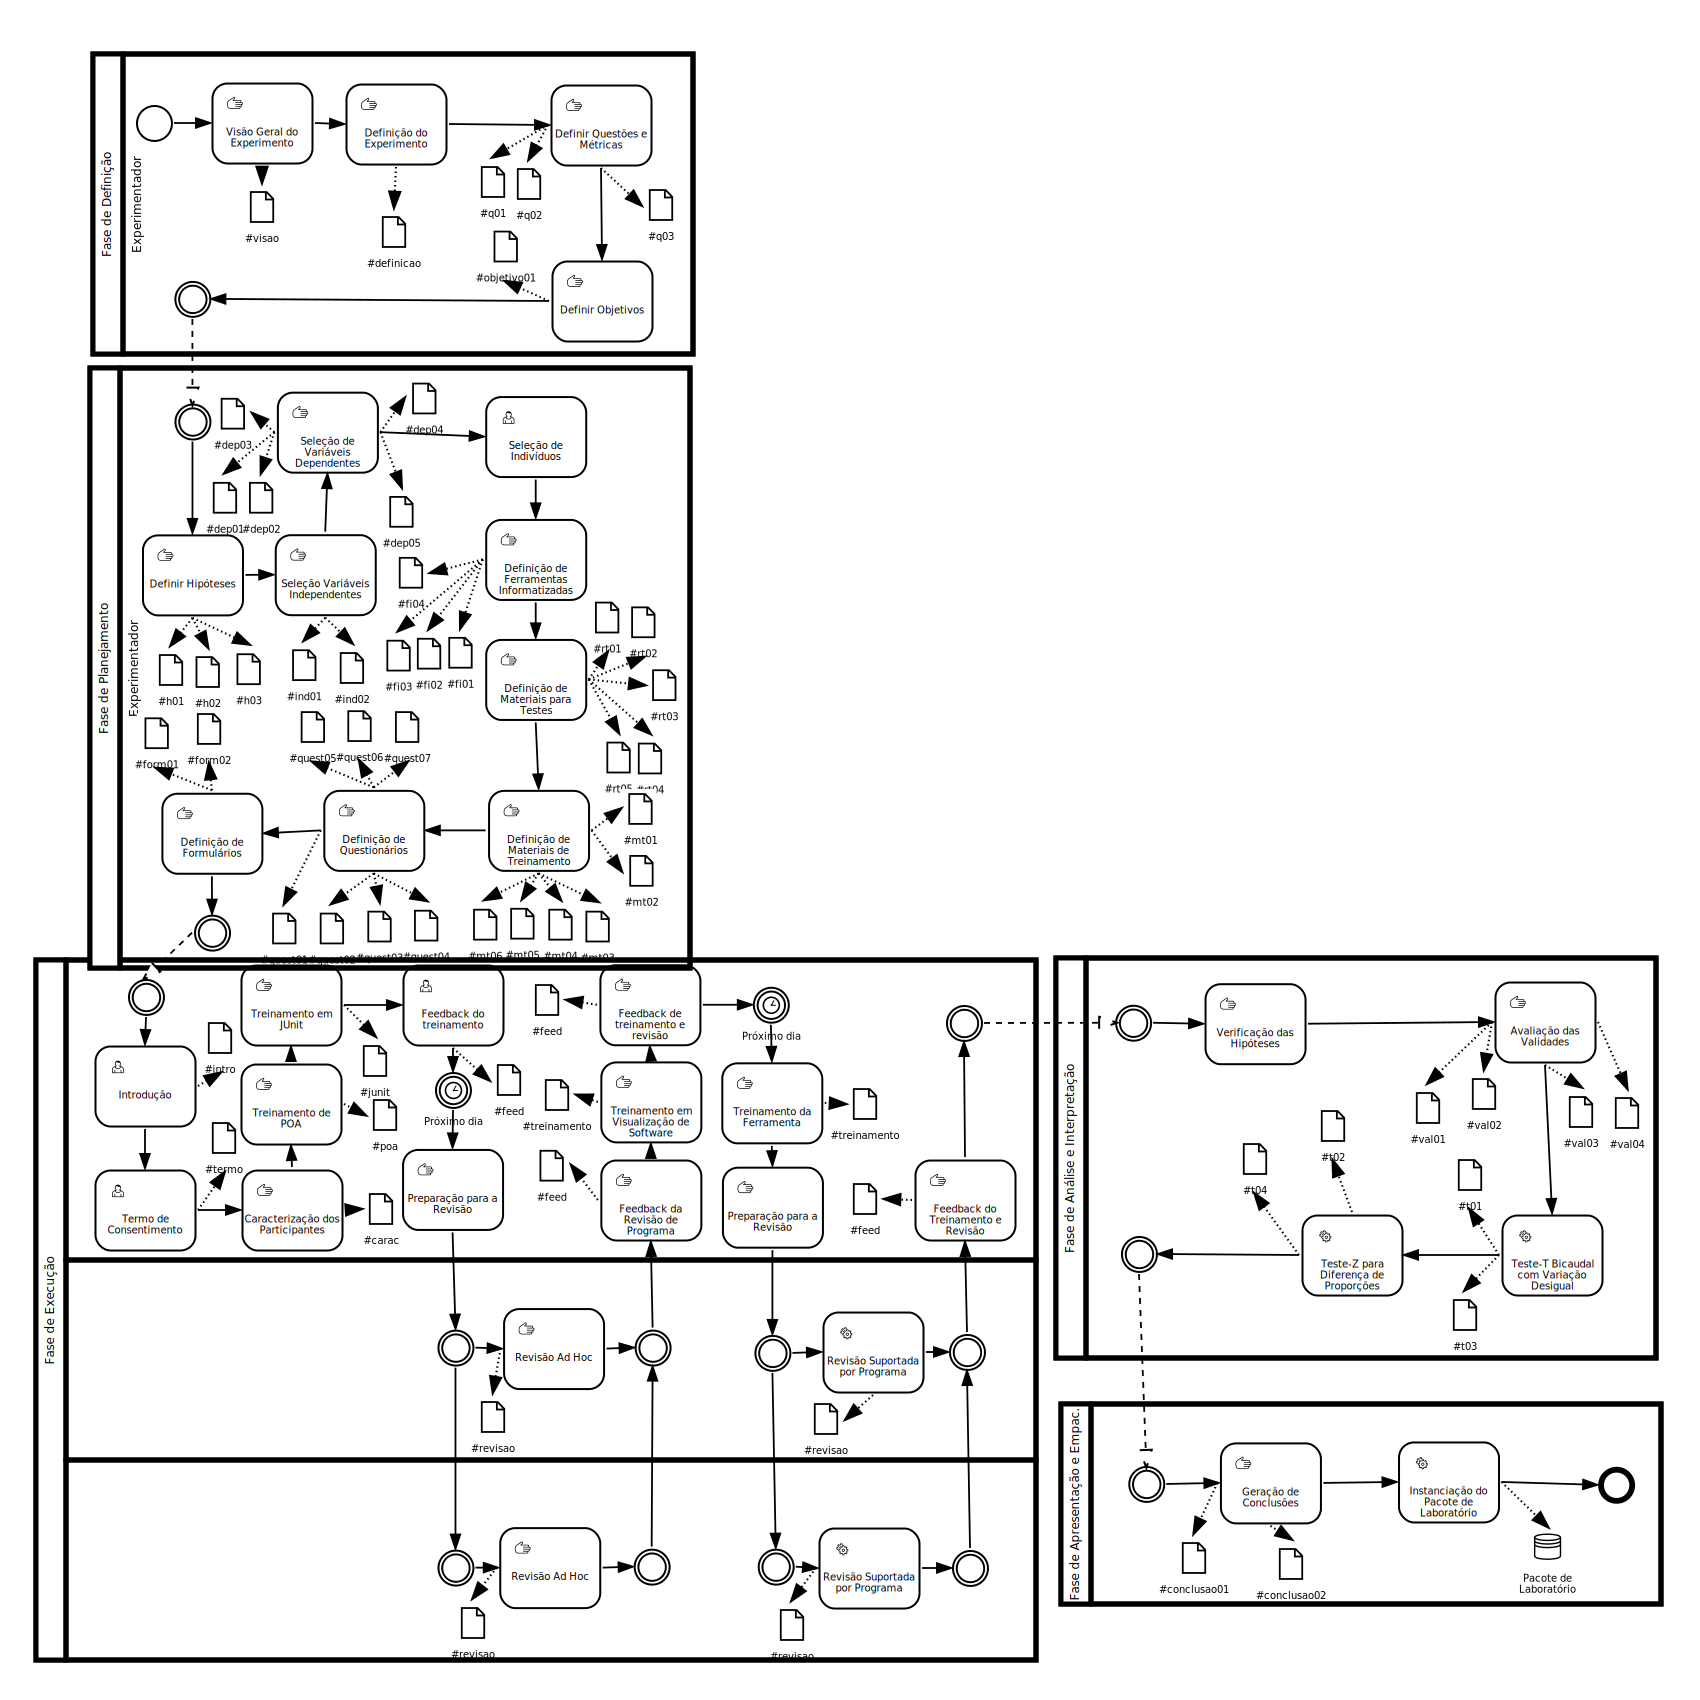
\includegraphics[scale=0.5]{images/diagrama.png}
\caption{Exemplo de diagrama BPMN – adaptado de \cite{Weske2012}.}
\label{diag}
\end{figure}

A Figura \ref{diag} apresenta, como exemplo, um simples diagrama de processo de negócio, através do qual é possível identificar a interação entre dois atores através da execução de atividades e trocas de mensagens, assim como, o uso de recursos como artefatos e repositórios de dados.

A especificação completa da atual versão define atributos que são agrupados em quatro categorias básicas de elementos: objetos de fluxo (\textit{Flow Objects}), objetos de conexão (\textit{Connecting Objects}), vias (\textit{Swimlanes}) e artefatos (\textit{Artifacts}). 
Na a Figura~\ref{elementos} há uma visão geral dos elementos da atual versão do BPMN.

\begin{figure}[!ht]
\centering
\includegraphics[scale=0.5]{images/elementos.png}
\caption{Conjunto de elementos que compõem a versão BPMN 2.0 \cite{object2016business}.}
\label{elementos}
\end{figure}

\section{Protocolos de experimentação usando BPM}

Compreender o projeto do experimento e revisar suas informações é fundamental não só para a execução do experimento, mas também para sua replicação. Diversos pesquisadores tem realizado projetos pilotos que ocasionam somente aumento de custos \cite{Kitchenham2008}. 

A utilização da notação de processo de negócio pode contribuir diretamente tanto na concepção quanto na execução do protocolo de estudo experimental. Primeiramente, devido à facilidade de compreensão do uso que compõem a respectiva notação, principalmente pelo fato de consistir em um padrão UML. Em segundo ponto, a utilização de pacotes de laboratório para o armazenamento das informações relativas aos protocolos realizados em cada experimento.

Através destes modelos de processo a seguir, é possível observar a sequência de execução das atividades, os fatores limitantes, tais como tempo, e também a estruturação de cada um dos processos e suas subdivisões.

Nas figuras \ref{selecao}, \ref{g1} e \ref{g2} são apresentados os diagramas de processo de negócio referentes ao protocolo de experimentação aplicado como parte do projeto de mestrado entitulado ``ModelUI$_{VIZ}$ - Uma proposta para representação de modelos de interface do usuário utilizando Visualização de Informação'', sob responsabilidade de Livia Cristina Gabos Martins, participante do Laboratório de Pesquisa em Engenharia de Software Aplicada -- LaPESA.

A representação do modelo de diagrama de processo de negócio também deve ser armazenado no pacote de laboratório, viabilizando o compartilhamento do protocolo juntamente com os dados referentes ao experimento, tais como hipóteses, variavéis dependentes e independentes.

%%%%%%%%%%%%%% selecao grupos
\begin{figure}[!ht]
\centering
\includegraphics[scale=0.7]{images/selecao.png}
\caption{Processo de atribuição de participantes aos grupos.}
\label{selecao}
\end{figure}


\begin{landscape}

%%%%%%%%%%%%%% grupo 01
\begin{figure}[!ht]
\centering
\includegraphics[scale=0.7]{images/grupo01.png}
\caption{Diagrama BPM referente às atividades dos participantes do primeiro grupo.}
\label{g1}
\end{figure}



%%%%%%%%%%%%%%% grupo 02
\begin{figure}[!ht]
\centering
\includegraphics[scale=0.7]{images/grupo02.png}
\caption{Diagrama BPM referente às atividades dos participantes do segundo grupo.}
\label{g2}
\end{figure}


\end{landscape}





	
	\chapter{Protótipo da Interface de Modelagem}
\label{cp:prototipo}

Neste capítulo é apresentada a interface da implementação parcial (situação atual do desenvolvimento) tanto da camada de interface para modelagem gráfica quanto da camada de persistência para a notação.
Primeiramente, em relação à camada de interface, trata-se de uma plataforma \textit{web} e, para sua implementação, foram utilizados a linguagem de marcação HTML 5 (\textit{HyperText Markup Language}), o CSS 3 (\textit{Cascading Style Sheets}) e a linguagem \textit{JavaScript}. Adicionalmente, as bibliotecas \textit{JQuery} e \textit{SVGPanZoom} são utilizadas para facilitar a implementação de recursos gráficos e execução de requisições HTTP/Ajax para a comunicação com o servidor, e manipulação dos elementos gráficos por meio de de operações de escala e deslocamento, respectivamente.

A ferramenta foi projetada para ser simples e intuitiva, com foco na elaboração dos diagramas. A página inicial é apresentada na Figura~\ref{inicial}.

\begin{figure}[!htb]
\centering
\includegraphics[width=\textwidth]{images/ferramenta.png}
\caption{Interface de modelagem da notação.}
\label{inicial}
\end{figure}

Para a criação de um novo modelo de diagrama de processo de negócio, é necessário somente realizar a inserção dos componentes do diagrama, ou caso já haja um modelo representado, o usuário deve selecionar a opção \textit{"Menu -> New"} para iniciar a representação. O menu da ferramenta é apresentado na Figura~\ref{menu}.

\begin{figure}[!htb]
\centering
\includegraphics[scale=0.75]{images/menu.png}
\caption{Menu de opções da ferramenta.}
\label{menu}
\end{figure}

Ainda em relação à Figura~\ref{menu}, é possível observar outras opções. Na opção \textit{``Menu -> Open''}, o usuário abrir um modelo de processo de negócio elaborado previamente nesta ferramenta, armazenados em arquivos com a extensão \textit{.bpmn}. A opção ``\textit{Menu -> Save as''} permite o armazenamento do modelo no mesmo formato citado anteriormente, sendo este um diagrama concluído ou em processo de criação. Por fim, a opção \textit{``Menu -> Export''} visa armazenar o modelo em formato de imagem vetorial, no formato SVG (\textit{Scalable Vector Graphics}), de forma que, o usuário, mesmo sem acesso a esta ferramenta, possa ter acesso ao conteúdo do modelo, ao menos, para leitura de seu conteúdo.

Para a construção do modelo de processo de negócio, o usuário faz uso de elementos tais como: \textit{Events}, \textit{Gateways}, \textit{Tasks}, \textit{Pools/Lanes}, \textit{Data Objects} e \textit{TextAnnotations}. Estes elementos são encontrados na ferramenta pelo menu lateral, no qual estão presentes todos os itens dessa categorias listas anteriormente.

Na Figura~\ref{eventos}, todos os eventos e suas derivações são listados.

\begin{figure}[!htb]
\centering
\includegraphics[scale=0.75]{images/eventos.png}
\caption{Painel de elementos da categoria de eventos.}
\label{eventos}
\end{figure}

Na Figura~\ref{gate} são apresentados os elementos que compõem a categoria de portões. E na Figura~\ref{lane} são exibidos os elementos referentes a piscinas e raias.

\begin{figure}[!htb]
\centering
\subfigure[Categoria de \textit{gateways}\label{gate}]{\includegraphics[scale=0.75]{images/gate.png}}\qquad\qquad
\subfigure[Categoria de piscinas e raias\label{lane}]{\includegraphics[scale=0.75]{images/lane.png}}
\caption{Painel de elementos}
\label{elementos}
\end{figure}
%\includegraphics[scale=0.75]{images/gate.png}




Cada elemento pertencente à notação será persistido no formato XML para composição do pacote de laboratório. A figura~\ref{mensagem} representa uma tarefa da categoria de mensagens, este elemento será armazenamento no modelo apresentado na listagem~\ref{ls:message}

\begin{figure}[!htb]
\centering
\includegraphics[scale=0.75]{images/mensagem.jpg}
\caption{Exemplo de elemento \textit{MessageTask}.}
\label{mensagem}
\end{figure}

\lstset{language=XML}
\begin{lstlisting}[caption=Descrição do elemento \textit{Mensagem}, label=ls:message]
<messagetask id="23">
	<type>task</type>
	<from>15</from>
	<to>42</to>
	<value>Download XML Files</value>
</messagetask>
\end{lstlisting}

Em relação ao servidor da plataforma \textit{web} em desenvolvimento, está sendo utilizada a linguagem de programação \textit{Java}, o servidor \textit{GlassFish Server 4.1} e o JSP - \textit{Java Server Pages}. Adicionalmente, para o suporte à serialização dos dados no formato XML (\textit{eXtensible Markup Language}) é utilizada a biblioteca \textit{XStream}. Esta parte da aplicação provê suporte tanto à leitura e escrita dos arquivos, quanto à validação dos diagramas, em termos de completude e corretitude, e também a extração do conteúdo de pacotes de laboratório e criação do respectivo modelo de processo. Aliás, a estrutura do arquivo XML deverá conter tanto elementos para representar o modelo visual BPMN (como coordenadas para posicionamento de elementos gráficos na interface), quanto elementos que representam os conceitos do Pacote de Laboratório.

Atualmente, em relação à camada de persistência, todos os elementos compõem a primeira versão da notação já foram implementados, e está em andamento a implementação dos elementos da segunda versão da notação BPM. Atualmente, foram implementadas trinta e uma classes, divididas em seis pacotes conforme a categorização dos elementos da notação. Tem sido adotada uma abordagem evolutiva, portanto os diagramas, assim como o modelo de classes, têm sido, também, alvo de contante evolução.


A seguir, na Listagem\ref{lst:classe} é apresentada a classe \textit{BusinessProcessDiagram} (apenas dados privados, que devem ser armazenados), a qual representa o componente básico de um diagrama BPMN, sendo responsável pela organização de todo o diagrama. O armazenamento desse elemento em pacote de laboratório está representado na Listagem~\ref{xml}.

\lstset{language=java}
\begin{lstlisting}[caption=Estrutura de Dados inicial da classe diagrama BPM, label=lst:classe]
public class BusinessProcessDiagram {
    private String id; 
    private String name; 
    private String version; 
    private String author; 
    private String language;  
    private String queryLanguage; 
    private Date creationDate;
    private Date modificationDate; 
    private ArrayList<Pool> pools; 
    private String documentation; 
}
\end{lstlisting}


\lstset{language=XML}
\begin{lstlisting}[caption=Estrutura do XML da classe diagrama BPM, label=xml]
<businessprocessdiagram id="1245" name="Selecao dos grupos">
  <author>Leandro Ungari</author>
  <language>pt-br</language>
  <queryLanguage>BPMN</queryLanguage>
  <creationDate>01/05/2017</creationDate>
  <modificationDate>10/05/2017</modificationDate>
  <pools>
    <pool id="1">...</pool>
    <pool id="2">...</pool>
    <pool id="3">...</pool>
         ...
    <pool id="n">...</pool>
  </pools>
  <documentation>Elemento formalizado pela documentacao BPMN 2.0 ...
	</documentation>
</businessprocessdiagram>
\end{lstlisting}





	
	\chapter{Construção de Protocolo de Experimentação}
\label{cp:construcao}

Neste capítulo é demonstrado o processo de construção de um protocolo de experimentação utilizando a ferramenta implementada neste trabalho, de modo a ilustrar o apoio que esta provê ao experimentador em cada fase do processo experimental, descrito pela Figura~\ref{ideia}. A apresentação é demonstrada de forma individual para cada fase: \textit{Definição}, \textit{Planejamento}, \textit{Operação}, \textit{Análise} e \textit{Empacotamento}.

Para a condução desta demonstração foi escolhido o experimento conduzido para avaliar a eficácia e a eficiência da Ferramenta de Visualização de Software \textit{SofVisOAH}~\cite{d2012avaliaccao}. Os dados que compõem o Pacote de Laboratório desse estudo foram utilizados para a instanciação do Pacote de Laboratório utilizando a ferramenta BPMN implementada neste trabalho.

\section{Experimento de Demonstração: Avaliação da \textit{SofVisOAH}}

O respectivo experimento de demonstração refere-se ao trabalho de ~\citeauthoronline{d2012avaliaccao}~(\citeyear{d2012avaliaccao}), que contextualiza como auxílio à área de Engenharia de Software, a Visualização de Software, a qual lida com a complexidade estrutural, apoiando tarefas de Compreensão de Programas por meio de representações visuais, permitindo interação com essas representações gráficas, provendo auxílio ao processo de entendimento. Uma ferramenta de Visualização de Software proporciona suporte ao usuário para obter informações por meio de análises dos artefatos visuais disponíveis, gerando assim, auxílio ao processo de entendimento de programas~\cite{d2012avaliaccao}.

O principal objetivo do experimento de ~\citeauthoronline{d2012avaliaccao}~(\citeyear{d2012avaliaccao}) é avaliar a utilização da ferramenta \textit{SofVisOAH} no apoio ao entendimento de Programas Orientados
a Aspectos, em detrimento ao entendimento de código convencional. Alguns fatores foram avaliados no experimento: verificação se a ferramenta auxilia na localização de defeitos assim como a compreensão de um Programa Orientado a Aspectos~\cite{d2012avaliaccao}.

Com a condução do experimento, os participantes puderam fornecer como respostas, além das medições que permitiram derivar métricas quantitativas relativas ao uso da ferramenta, uma avaliação qualitativa da mesma. Após a condução do experimento e avaliação dos resultados, foi possível constatar estatisticamente que a \textit{SofVisOAH} proveu auxílio às tarefas de Localização de Defeitos e Compreensão de Programa~\cite{d2012avaliaccao}.

\section{Elaboração do Protocolo de Experimentação}

\subsection{Fase de Definição}
Inicialmente devem ser definida uma visão geral relativa experimentação através dos itens estão descritos a seguir~\cite{d2012avaliaccao}:

\begin{itemize}

\item Objeto de Estudo -- Ferramenta de Visualização de Software \textit{SofVisOAH}.

\item Propósito -- avaliar e comparar a utilização da ferramenta \textit{SofVisOAH} como apoio a tarefas de Revisão de Programa em relação à Revisão de Programa Ad Hoc.

\item Enfoque de Qualidade -- Tempo, Quantidade de defeitos localizados e Entendimento do programa.

\item Perspectiva -- Do experimentador.

\item Contexto -- Laboratório de informática da Universidade Estadual Paulista Júlio de Mesquita Filho, Unesp, no campus da Faculdade de Ciências e Tecnologia.

\end{itemize}

A elaboração do modelo de processo de negócio, representado na Figura~\ref{img:protocolo-definicao}, explicita a sequência de atividades (Definir Objeto de Estudo, Definir Propósito, Definir Métrica, Definir Perspectiva e Definir Contexto) que devem ser executadas para a definição dos itens descritos acima, e seus respectivos artefatos produzidos. Todas as atividades executadas neste processo foram realizadas pelo Experimentador.

%figura DEFINICAO
\begin{figure}[!htb]
\centering
\includegraphics[width=0.85\textwidth]{images/protocolo-definicao.png}
\caption{Protocolo de Experimentação referente à Fase de Definição.}
\label{img:protocolo-definicao}
\end{figure}

A construção do processo referido na Figura~\ref{img:protocolo-definicao}, a partir da adição da piscina referente a Fase de Definição, é inserido o evento de início juntamente com as atividades listadas anteriormente, como cada atividade será executada pelo experimentador, essas devem ser da categoria \textit{User Task}. Por fim, a partir de cada atividade foram produzidos \textit{Data Objects} referentes as definições estabelecidas.

\subsection{Fase de Planejamento}
Na fase seguinte, devem ser definidos um conjunto de elementos de forma específica, dentre os quais: conjunto de questões e métricas (Figura~\ref{img:questoes}). Também foram planejadas hipóteses nulas e alternativas, ilustradas na Figura~\ref{img:hipoteses}, assim como, variáveis independentes (Figura~\ref{img:independentes}) e variáveis dependentes (Figura~\ref{img:dependentes})~\cite{d2012avaliaccao}.

%figura questoes
\begin{figure}[!htb]
\centering
\includegraphics[width=0.9\textwidth]{images/tabela-questoes.png}
\caption{Questões e Métricas elaboradas na Atividade Planejamento~\cite{d2012avaliaccao}.}
\label{img:questoes}
\end{figure}

%figura hipotese
\begin{figure}[!htb]
\centering
\includegraphics[width=0.9\textwidth]{images/tabela-hipoteses.png}
\caption{Hipóteses elaboradas na Atividade Planejamento~\cite{d2012avaliaccao}.}
\label{img:hipoteses}
\end{figure}

%figura independentes
\begin{figure}[!htb]
\centering
\includegraphics[width=0.9\textwidth]{images/tabelas-variaveis-independentes.png}
\caption{Variáveis Independentes elaboradas na Atividade Planejamento~\cite{d2012avaliaccao}.}
\label{img:independentes}
\end{figure}


%figura dependentes
\begin{figure}[!htb]
\centering
\includegraphics[width=0.9\textwidth]{images/tabelas-variaveis-dependentes.png}
\caption{Variáveis Dependentes elaboradas na Atividade Planejamento~\cite{d2012avaliaccao}.}
\label{img:dependentes}
\end{figure}


Em seguida, a Seleção de Participantes, os quais são escolhidos mediante seleção determinística, envolvendo alunos de graduação em Ciência da Computação~\cite{d2012avaliaccao}.

Por fim, foi definida a instrumentação, categorizada em dois tipos: Tecnologia e Artefato. Os instrumentos de Tecnologia foram definidos de acordo com os requisitos tecnológicos para a execução de ambas as revisões de programa e conhecimento prévio para a realização das mesmas. A instrumentação é dividida nos seguintes grupos: Ferramentas Informatizadas (Figura ~\ref{img:instrumentacao1}), Materiais de Realização de Testes (Figura~\ref{img:instrumentacao2}), Materiais de Treinamento (Figura~\ref{img:instrumentacao3}), Questionários (Figura~\ref{img:instrumentacao4}) e Formulários (Figura~\ref{img:instrumentacao5})~\cite{d2012avaliaccao}.

%figura
\begin{figure}[!htb]
\centering
\includegraphics[width=0.9\textwidth]{images/tabela-instrumentacao1.png}
\caption{Instrumentação – Ferramentas Informatizadas – Planejamento~\cite{d2012avaliaccao}.}
\label{img:instrumentacao1}
\end{figure}

%figura
\begin{figure}[!htb]
\centering
\includegraphics[width=0.9\textwidth]{images/tabela-instrumentacao2.png}
\caption{Instrumentação – Materiais de Realizacao de Testes – Planejamento~\cite{d2012avaliaccao}.}
\label{img:instrumentacao2}
\end{figure}

%figura
\begin{figure}[!htb]
\centering
\includegraphics[width=0.9\textwidth]{images/tabela-instrumentacao3.png}
\caption{Instrumentação – Materiais de Treinamento – Planejamento~\cite{d2012avaliaccao}.}
\label{img:instrumentacao3}
\end{figure}

%figura
\begin{figure}[!htb]
\centering
\includegraphics[width=0.9\textwidth]{images/tabela-instrumentacao4.png}
\caption{Instrumentação – Questionários – Planejamento~\cite{d2012avaliaccao}.}
\label{img:instrumentacao4}
\end{figure}

%figura
\begin{figure}[!htb]
\centering
\includegraphics[width=0.9\textwidth]{images/tabela-instrumentacao5.png}
\caption{Instrumentação – Formulários – Planejamento~\cite{d2012avaliaccao}.}
\label{img:instrumentacao5}
\end{figure}

%%%%%%%%%%%%
%%%%%%%%%%%%
%figura PLANEJAMENTO
\begin{figure}[!htb]
\centering
\includegraphics[width=0.85\textwidth]{images/protocolo-planejamento.png}
\caption{Protocolo de Experimentação referente à Fase de Planejamento.}
\label{img:protocolo-planejamento}
\end{figure}


O plano de execução da \textit{Fase de Planejamento}, representada pelo modelo de processo de negócio apresentado na Figura~\ref{img:protocolo-planejamento}, define as atividades a seguir: Definição das Questões e Métricas (visa a elaborar o que será avaliado e como será medido), Elaboração das Hipóteses (objetiva definir a efetividade da ferramenta sob as suposições), Definição das Variáveis Dependentes e Independentes (define quais fatores podem influenciar de forma direta e indireta e como estes serão tratados), e por fim, Definição da Instrumentação (define os instrumentos que serão utilizados no experimento como ferramentas de software, apresentações visuais, questionários e formulários). Todas as atividades desta fase são executadas pelo Experimentador.

A construção do diagrama referente a esta fase, representado na Figura~\ref{img:protocolo-planejamento}, inicia-se a partir da inserção da piscina referente a Fase de Planejamento e do evento de início. Em seguida, são adicionadas as atividades do tipo \textit{User Task}, pois todas atividades desta fase são referentes ao usuário, e por fim o evento de término. A partir destas atividades foram produzidos \textit{Data Objects} referentes às questões e métricas, hipóteses nulas e alternativas, variáveis dependentes e independentes e diversos artefatos, tais como formulários, questões, treinamentos, testes e ferramentas.

\subsection{Fase de Operação}
Para a execução deste experimento, o conjunto de participantes foi aleatoriamente dividido em dois grupos: os participantes de código ímpar foram alocados para o Grupo A e os demais para o Grupo B. Cada participante teve seu perfil caracterizado por meio de um questionário de levantamento de perfil através da \textit{OntoExpTool}. Os participantes realizaram os mesmos tipos de atividade, revisões de programa Ad Hoc e com o apoio da ferramenta \textit{SofVisOAH}, exercendo entendimento do programa e a localização de defeitos no código fonte~\cite{d2012avaliaccao}.

%%%%%%%%%%%%
%%%%%%%%%%%%
%figura OPERACAO
\begin{figure}[!htb]
\centering
\includegraphics[width=0.85\textwidth]{images/protocolo-operacao.png}
\caption{Protocolo de Experimentação referente à Fase de Operação.}
\label{img:protocolo-operacao}
\end{figure}

Para esta fase, o modelo de processo respectivo, apresentado na Figura~\ref{img:protocolo-operacao}, define a execução de três processos relacionados. O primeiro, sob responsabilidade do Experimentador é composta pelas atividades: Aplicação de Questionários de Perfil (para todos os participantes são aplicadas questões sobre perfil, assim como do treinamento e revisão do programa) e Seleção de Grupos (separação dos participantes entre os dois grupos definidos). A partir da finalização do processo anterior, são iniciados os processos referentes aos participantes do Grupo A e B de forma concomitante, contendo as seguintes tarefas de forma alternada: Análise AdHoc (realiza-se o processo de detecção de defeitos sem qualquer auxílio automatizado) e Análise Apoiada (realiza-se a detecção de defeitos com o auxílio das técnicas de visualização apresentadas na ferramenta \textit{SofVisOAH}).

Em relação a construção do protocolo apresentado na Figura~\ref{img:protocolo-operacao}, inicialmente adiciona-se a piscina referente à Fase Operação, em seguida esta é dividida em três partes, uma cada categoria de atores. A execução inicia-se por meio da aplicação do questionário e seleção de grupos realizada pelo experimentador, logo, são adicionadas atividades para cada tarefa na parte referente ao experimentador. Após, são adicionadas as atividades de análise apoiada e Ad Hoc para cada grupo de modo alternado. Por fim, são adicionados os eventos de término.


\subsection{Fase de Análise e Interpretação}

Na análise executada no experimento, os participantes descreveram corretamente mais adendos de aspectos utilizando a \textit{SofVisOAH}. Em relação ao quesito auxílio à Compreensão de Programa, foi aplicado o Teste-T Bicaudal com Variação Desigual. Portanto, constata-se que a utilização da ferramenta provê auxílio à Compreensão de Programa~\cite{d2012avaliaccao}.

%%%%%%%%%%%%
%%%%%%%%%%%%
%figura ANALISE
\begin{figure}[!htb]
\centering
\includegraphics[width=0.85\textwidth]{images/protocolo-analise.png}
\caption{Protocolo de Experimentação referente à Fase de Análise e Interpretação.}
\label{img:protocolo-analise}
\end{figure}

Desse modo, a elaboração do modelo de processo, ilustrado na Figura~\ref{img:protocolo-analise} é composta pelas seguintes atividades, todas estas executadas pelo Experimentador: Avaliação da Descrição dos Participantes (foi realizada a extração dos dados coletados a partir de questionários e formulários sobre o perfil do participante e a ferramenta \textit{SofVisOAH}), Aplicação do Método Estatístico (a partir do conjunto de dados foi aplicado o Teste-T) e Geração de Conclusões (através da finalização do teste estatístico juntamente com as hipóteses e variáveis definidas foi estabelecido o conjunto de conclusões sobre o objeto em investigação).

Para esta fase, a elaboração do protocolo de experimentação (Figura~\ref{img:protocolo-analise}), inicia-se com a adição do piscina e do início de evento e seguido das respectivas atividades indicadas. Como entrada do processo, indicado pelo \textit{Data Input} têm-se os dados coletados na fase anterior, os quais são vinculados com a primeira atividade. Como resultado da terceira atividade foram obtidas as conclusões do estudo, indicadas por meio de um \textit{Data Output}. De modo a encerrar, adiciona-se o evento de término.


\subsection{Fase de Empacotamento e Apresentação}

Como último passo, a \textit{Fase de Empacotamento e Apresentação}, os dados de todo o transcorrer do experimento foram armazenados em uma base de dados e após da fase anterior, o Pacote de Laboratório deste experimento foi instanciado em dois formatos: XML e OWL, permitindo ser visualizados na própria ferramenta~\cite{d2012avaliaccao}.

Também foi criado um pacote compactado contendo o	s arquivos descritos acima, e todos os artefatos e documentos provenientes do estudo, desse modo, disponíveis para análises e futuras replicações~\cite{d2012avaliaccao}. 

%%%%%%%%%%%%
%%%%%%%%%%%%
%figura EMPACOTAMENTO
\begin{figure}[!htb]
\centering
\includegraphics[width=0.85\textwidth]{images/protocolo-empacotamento.png}
\caption{Protocolo de Experimentação referente à Fase de Empacotamento e Apresentação.}
\label{img:protocolo-empacotamento}
\end{figure}

Por fim, o modelo de processo de negócio (ilustrado na Figura~\ref{img:protocolo-empacotamento}) representa o protocolo de execução da \textit{Fase de Empacotamento e Apresentação}, que neste experimento é composta pela seguintes atividades: Armazenamento na Base de Dados (são obtidos todos os conjuntos de dados gerados nas atividades das fases anteriores), Exportação dos Arquivos OWL e XML (processamento e geração destes arquivos) e, Instanciação do Pacote de Laboratório (encapsulamento dos dados relativos ao experimento juntamente com todos seus artefatos), todas atividades executadas pelo Experimentador.

O plano de execução referente a essa etapa, inicia-se a partir da adição da piscina dessa fase e o início de evento. Em seguida, foram adicionadas atividades automatizadas (\textit{Script Task}), para o armazenamento dos dados em um Banco de Dados e na forma de Pacote de Laboratório, ambos representados por \textit{Data Store}. Concluindo, é adicionado o evento de término.

\section{Considerações Finais}
Neste capítulo foi apresentado o processo de concepção do protocolo de experimentação (plano de execução) em experimentos controlados. A partir da realização das atividades em cada fase, novos componentes são atrelados ao corpo de experimento, em que a partir de versões iniciais são refinados nas fases subsequentes, por exemplo, o conjunto de hipóteses que foi definido e aprimorado nas fases de Definição e Planejamento, respectivamente, também está presente na fase de Análise e Interpretação atuando como uma entrada de dados para esta fase.
Além disso, é possível perceber as relações e dependências entre atividades de diferentes fases do estudo experimental.
	
	%\chapter{Plano inicial e atividades realizadas}
\label{ch:plano_atividades}

\section{Cronograma Inicial}
O cronograma de atividades foi organizado de acordo com a Tabela ~\ref{tab_cronograma}. As atividades foram divididas mensalmente, com início em dezembro de 2016. Nessa tabela as letras 'x' correspondem às atividades previstas, 'X' às atividades já realizadas e os símbolos '-' às atividades em execução.

\begin{itemize}
\item \textit{Atividade 1}: Revisão Bibliográfica (e da tecnologia a ser utilizada);
\item \textit{Atividade 2}: Definição dos requisitos da camada de interface;
\item \textit{Atividade 3}: Desenvolvimento da camada de interface;
\item \textit{Atividade 4}: Avaliação da interface desenvolvida;
\item \textit{Atividade 5}: Relatório Parcial;
\item \textit{Atividade 6}: Relatório Final.

\end{itemize}


\begin{table}[htbp]
\centering 
\caption{Cronograma de Atividades}
\label{tab_cronograma}
\small
\begin{tabular}
{|c|c|c|c|c|c|c|c|c|c|c|c|c|} \cline{2-13}
\multicolumn{1}{c|}{}&\multicolumn{12}{c|}{\textbf{Período}}
 \\
\cline{2-13}
\multicolumn{1}{c|}{}&\multicolumn{1}{c|}{\textbf{2016}} &\multicolumn{11}{c|}{\textbf{2017}} \\
\hline Atividades & Dez & Jan & Fev & Mar & Abr & Mai & Jun & Jul & Ago & Set & Out & Nov \\
\hline         1  & X   & X   &  X  &  X  &     &     &     &     &     &     &     &     \\
\hline         2  &     &     &  X  &  X  &     &     &     &     &     &     &     &     \\
\hline         3  &     &     &     &  X  &  X  &  X  &  X  &  X  &  X  &     &     &     \\
\hline         4  &     &     &     &     &     &     &     &     &  -  &  -  &  -  &  -  \\
\hline         5  &     &     &     &     &     &  X  &     &     &     &     &     &     \\
\hline         6  &     &     &     &     &     &     &     &     &     &     &  X  &  X  \\
\hline
\end{tabular}
\normalsize
\end{table}

\section{Atividades Realizadas}

Conforme estabelecido pelo cronograma inicial, as atividades previstas para a primeira parte do projeto, anteriores a entrega do relatório científico parcial, tinham como propósito o embasamento teórico dentro do contexto da Engenharia de Software Experimental sobre experimentos controlados, o uso de pacotes de laboratório para transferência de dados entre grupos de pesquisa. Em seguida, iniciou-se o estudo sobre modelos de processo de negócio e suas notações para representação de modelos gráficos, em específico a BPMN.

Em seguida, a partir dos requisitos da camada de interface para modelagem, foi iniciada a implementação desta ferramenta de modo a viabilizar a construção dos modelos de processo de negócio com todos os elementos previstos pela documentação da notação em sua versão atual.

Após a elaboração desta interface de modelagem, foi iniciada a construção da camada de persistência dos modelos de processo, assim como a recuperação e armazenamento destes em documentos de forma permanente. De modo análogo também foi construída uma camada de persistência e uma interface de dados para obtenção dos conteúdos relativos aos experimentos executados e armazenados segundo o modelo proposto pela ontologia \textit{ExperOntology} a partir da ferramenta \textit{OntoExpTool}. Desse modo, a partir da leitura de um pacote de laboratório é possível incorporar o modelo processo de negócio respectivo ao experimento, e assim, incorporando o protocolo de experimentação.

Em seguida, foram estabelecidas avaliações para a detecção de inconsistências tanto na ferramenta quanto na representação da notação, e desta forma, suas devidas correções. Também foram construídos alguns modelos de diagramação de forma a representar os protocolos de estudos experimentais já previamente executados para avaliar se a notação apresentada supre todas as necessidades encontradas.

Por fim, foi iniciada a construção do presente relatório científico final.


	
	\chapter{Considerações Finais}
\label{cp:conclusoes}

Nessa primeira parte do projeto, além dos estudos teóricos, foi implementada a camada de persistência referente à primeira versão da respectiva notação, assim como classes e métodos auxiliares armazenar no formato \textit{XML}, conforme a estruturação de um pacote de laboratório. Paralelamente, tem sido desenvolvida a camada de interface para a construção dos diagramas de processo de negócio.

Para uma avaliação mais precisa do uso da notação BPM na elaboração de processo de elaboração de protocolos de experimentos, é necessária a conclusão das duas atividades citadas acima, assim como a transferência dos dados de um pacote de laboratório para a representação gráfica.

A continuidade das atividades corresponde ao encerramento da implementação da camada de persistência assim como da interface de modelagem. Em seguida, será estabelecida a integração da interface de modelagem BPM com a ferramenta \textit{OntoExpTool}, de modo a visualizar graficamente o protocolo do experimento armazenado no pacote de laboratório.

A execução das atividades do projeto está dentro do esperado, desse modo, a conclusão das atividades deve ocorrer dentro dos prazos estabelecidos, assim como a elaboração do relatório científico final deste projeto de iniciação científica.

	% ----------------------------------------------------------
	% ELEMENTOS PÓS-TEXTUAIS
	% ----------------------------------------------------------
	\postextual
	% ----------------------------------------------------------

	% ----------------------------------------------------------
	% Referências bibliográficas
	% ----------------------------------------------------------
\renewcommand{\bibname}{Referências Bibliográficas}

\bibliography{referencias/referencias}

	
\end{document}
